\documentclass[conference]{IEEEtran}
\usepackage{amsmath,amssymb,amsfonts}
\usepackage{xcolor}
\usepackage{tikz, tikz-3dplot}
\usetikzlibrary{arrows,backgrounds,decorations,decorations.pathmorphing,
positioning,fit,automata,shapes,snakes,patterns,plotmarks,calc,trees,arrows.meta}
\usepackage{color}
\usepackage{pgfplots}
\pgfplotsset{compat=newest}
\usepackage{pgfplotstable}

\begin{document}

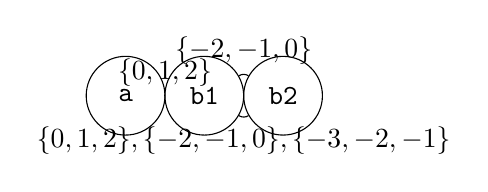
\begin{tikzpicture}
        
        % States
        \node[state, minimum size=1cm] (1) {\texttt{a}};
        \node[state, minimum size=1cm, right of=1] (2) {\texttt{b1}};
        \node[state, minimum size=1cm, right of=2] (3) {\texttt{b2}};
        
        % Edges
        \draw (2) edge node[above]{$\{0, 1, 2 \}$} (1);
        \draw (2) edge[bend right] node[below]{$\{0, 1, 2\}, \{-2, -1, 0\}, \{-3, -2, -1\}$} (3);
        \draw (3) edge[bend right] node[above]{$\{-2, -1, 0 \}$} (2);
        
    \end{tikzpicture}

\end{document}